\chapter{Electronics} % (fold)
\label{chap:electronics}
This chapter describes the construction of a number of sensor circuits using piezo electric elements to measure the time of arrival of bending waves.
\section{Design of comparator circuit for the piezo electrics elements}
This section describes the construction of a number of sensor circuits using piezo electric elements to measure the time of arrival of bending waves.

There is a circuit like the one on figure \ref{fig:print} for each sensor. It is chosen to make one print for each circuit in order to keep the wires conducting the analog sensor values as small as possible.
\begin{figure}[htb]
	\centering
	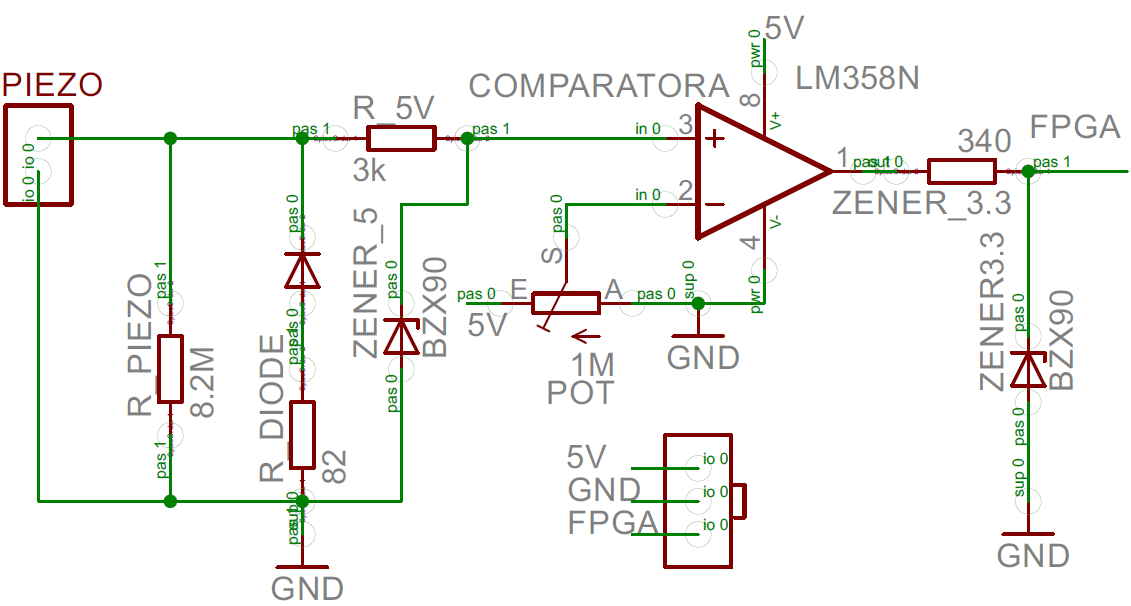
\includegraphics[width=.8\textwidth]{figures/Print}
	\caption{Schematics of circuit for digitalizing the output from a piezo electric elements.}
	\label{fig:print}
\end{figure}
The very small current that the piezo electric element generates are amplified with a resistor on $8.2\si{\ohm}$. This value is chosen since test showed that it was possible to detect ball bounce after a drop from a hight on $30\si{\centi\meter}$ which are deemed as the minimum drop hight.
Diodes are used to account for the large positive and negative voltage spikes that the sensor in combination with the large resistor can output in case of a powerful input to the sensor.
Since the negative voltage are not use it is removed up to $0.7V$ with a diode which conducts current from ground when the voltage from the piezo becomes less then $0.7V$.
The resistor to limit this current is calculated according to equation \ref{eq:distDifference}.
\begin{equation}
20 - 0.7 V = R_{diode} \cdot 300mA \Leftrightarrow R_{diode} = 64.3\si{\ohm}
\label{diodeResistor}
\end{equation}
The $20V$ is taken as a guess on the absolute maximum based on the fact that tests has not shown voltages above $15V$ when throwing the ball against the plate. Hence the system are robust against misuse. A resistor with a value above and close to $64.3\si{\ohm}$ that are available in stuck are used.
Since the op-amp cannot compare values that are larger than the supply of $5V$, the positive voltage is limited to $5.1V$ with a zener diode \cite{zener}. The resistor $R_5V$ is calculated by assuming infinite input resistance in the op-amp according to equation \ref{eq:zener5VResistor}.
\begin{equation}
%20 - 5 V = R_{5V} \cdot 5mA \Leftrightarrow R_{diode} = 3{k\si{\ohm}
\label{eq:zener5VResistor}
\end{equation}
A zener diode \cite{zener} is used to convert the $5V$ on the data output from the operational amplifier to $3.3V$, which is appropriate voltage for the FPGA. The solution with a zener diode is chosen over a another using a voltage divider since the voltage is kept at $3.3V$ for all op-amp's of the type LM358 even in cases of changes in production. According to the datasheet for LM358 the saturated output voltages varies from the supply voltages down to $1.5V$ below \cite{lm358}.
The resistor placed on the output of the operational amplifier is calculated using the current used for testing conditions in the datasheet for the diode, as can be seen in equation \ref{eq:zener} \cite{zener}.
\begin{equation}
5-3.3V = R_{z} I_{test} \Leftrightarrow R_{z} = 1.7V/5mA = 340\si{\ohm}
\label{eq:zener}
\end{equation}
%
A potentiometer is connected to the inverting pin of the op-amp in order to ease the tuning of the reference voltage. It's value is set to $1\si{\mega\ohm}$ to minimize the power consumption.
The tuning of the reference voltage is conducted by dropping a ball from $30\si{\centi\meter}$  and that the comparators are triggered. The voltage are lowered until the one off the sensor circuits does not detect the ball hit. Then it is raised to a bit above that to ensure detection. Hence the reference voltage for all of the four circuits are adjusted to $9.4V$ which have proven to be very robots against disturbances in the form of vibrations in the surrounding while still being able to detect ball hits.
%
\subsection{PCB Design and manufacturing}
After designing the schematics it was verified on a breadboard. Then the design from the breadboard are drawn as a schematics and a board in eagle.
The PCB is routed to keep wires as short as possible in order to minimize influence of noise as can be seen on figure \ref{fig:pcb}.
\begin{figure}[htb]
	\centering
	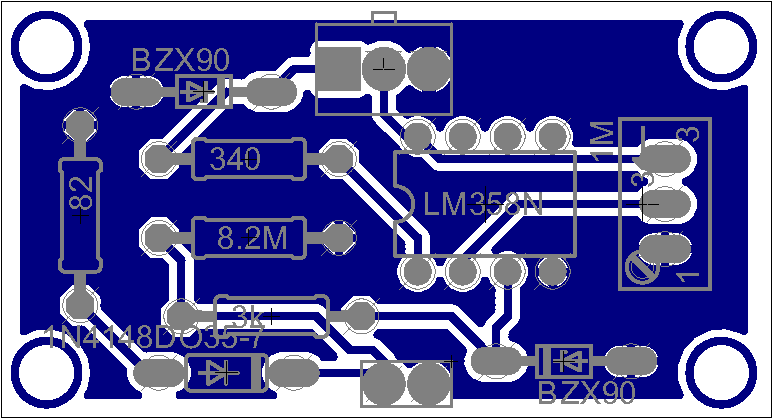
\includegraphics[width=.6\textwidth]{figures/pcb}
	\caption{PCB board of circuit for digitalizing the output from a piezo electric elements.}
	\label{fig:pcb}
\end{figure}
The width of the wires are chosen to be thick in order to ease the manufacturing. Then the risk of the wires disappearing in the basic fluid are smaller.
After verifying the schematics one of the four identical PCB's are manufactured and tested before producing the others.
Other simpler electrical connections are manufactured on stripboards to minimize time spend on producing PCB's.